\documentclass[titlepage]{article} % letter paper is implicit

\usepackage{siunitx} % for units
\usepackage{mathtools} % for amsmath
\usepackage{booktabs} % for better-looking tables
\usepackage{threeparttable} % for notes in tables
\usepackage[title]{appendix}
\usepackage{listings} % for source code
\usepackage{courier}
\usepackage[x11names]{xcolor} % for source code colors
\usepackage[moderate, % package to fit more text on a page, set moderate spacing
            mathspacing=normal, % keep horizontal spacing in math
            mathdisplays=normal, % keep vertical spacing around math
            leading=normal, % keep line spacing normal
            margins=tight, % allow custom margins (below)
            indent=normal,  % indent paragraphs normally
            marginwidth=1in]{savetrees} % set margin to 1in
\usepackage{biblatex} % For bibliography
\usepackage{amssymb} % For lists?
\usepackage{enumitem} % For lists?
\usepackage{tikz}  % FBDs with Plots
\usepackage{pgf} % Math printings
\usepackage{subcaption} % side by side figures
\usepackage{graphicx} % pictures
\usepackage{pdfpages} % drawings
% \setlength{\footskip}{30pt}

\sisetup{
    group-digits=integer,
    group-minimum-digits={3},
    group-separator={,},
    uncertainty-mode = separate,
    separate-uncertainty-units = single
}


\definecolor{codebackcolor}{rgb}{0.95,0.95,0.92}

\lstdefinestyle{myStyle}{
    backgroundcolor=\color{codebackcolor},   
    numberstyle=\tiny\color{gray},
    basicstyle=\ttfamily\footnotesize,
    identifierstyle=\color{Blue3},
    commentstyle=\color{SpringGreen4},
    keywordstyle=\color{Magenta3},
    stringstyle=\color{DarkOrange2},
    breakatwhitespace=false,         
    breaklines=true,                 
    keepspaces=true,                 
    numbers=left,       
    numbersep=5pt,                  
    showspaces=false,                
    showstringspaces=false,
    showtabs=false,                  
    tabsize=2,
}

\addbibresource{references.bib} % Import the bibliography file

\usetikzlibrary{backgrounds} % Plot Backgrounds
\usetikzlibrary{math} % Variables
\usetikzlibrary{patterns.meta} % cross hatch

\begin{document}

\title{Gearbox Design Report}
\author{Luke McGinnis\\Eastern Michigan University \\ME 330: Machine Design\\Dr. Emad Tanbour}

\date{April 21, 2025}

\maketitle

\tableofcontents

\begin{center}
    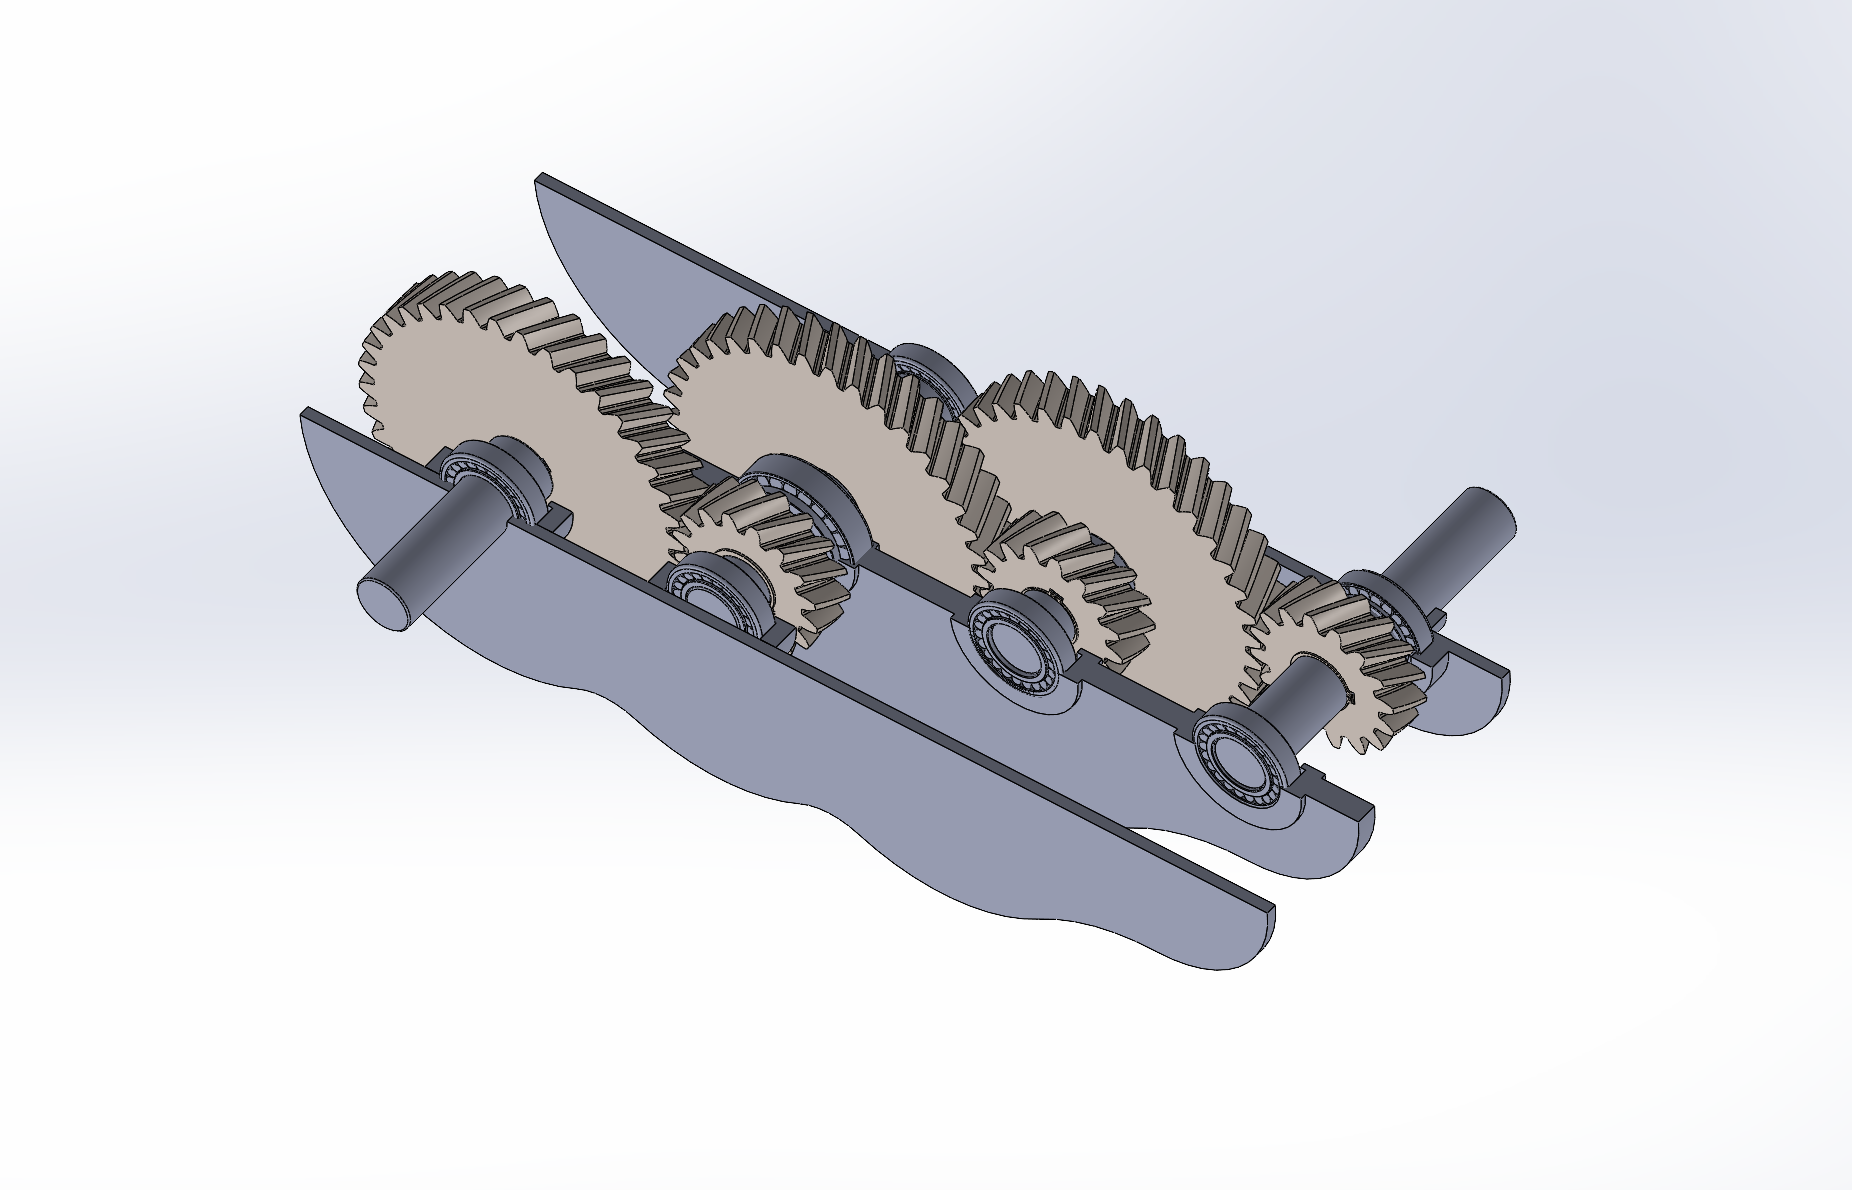
\includegraphics[width=0.75\textwidth]{figures/image.png}
\end{center}

\section{Introduction}

\subsection{Project Statement}
Using machine design principles, comprehensively design and create a CAD model
of a three-stage speed reduction gearbox. 

\subsection{Overall Requirements}
\begin{itemize}
    \item Reduce the shaft speed from an input of $\SI{1750}{rpm}$ to an output
    of $\SI{130(5)}{rpm}$.
    \item Tolerate an input power of $\SI{135}{hp}$.
    \item Consist of four shafts, one input, two intermediate, and one output.
    \item Use helical gears only.
    \item Be lubricated and sealed.
\end{itemize}

\subsection{Design Objectives}
\begin{itemize}
    \item Minimize the total size of the gearbox.
    \item Ensure the gearbox is easy to assemble and disassemble.
    \item Ensure manufacturability of all components.
\end{itemize}

\subsection{Methods}
\begin{itemize}
    \item Design report will be prepared with \LaTeX.
    \item CAD models, assemblies, drawing, simulations, and rendering will be
    prepared with Solidworks. 
\end{itemize}


\section{Gears Specifications}

\subsection{Requirements}
\begin{itemize}
    \item Overall gear train must convert $\SI{1750}{rpm}$ to $\SI{130(5)}{rpm}$.
    \item Gear train must handle an input power of $\SI{135}{hp}$.
    \item Gear train must be as compact as possible.
    \item All gears must be helical.
    \item Gears must be designed for a service life of \num{2000} hours per year
    and 6 years (\num{12000} hours total).
    \item Gears will be lubricated.
    \item AGMA (American Gear Manufacturers Association) design methodology will
    be used.
\end{itemize}

\subsection{Design Decisions}
\begin{itemize}
    \item All gears will use a standard pressure angle of \ang{20}. This is the
    most common pressure angle used for gearing and thus tooth cutters will be
    available for the greatest number of diametral pitches \cite{shigleydesign}.
    \item All gears will have full-depth teeth.
    \item All gears will have a helix angle of \ang{30}. This will allow for
    maximum advantage of strength and noise benefits of helical gears.
\end{itemize}

\subsection{Gear Ratio}
In order to achieve the smallest overall package size, we want our three stage 
ratios to be as close together as possible. Our requirements allow us to deviate
from our target output speed of \SI{130}{rpm} by as much as \SI{5}{rpm}. If we
assume the ideal case of all stage ratios being equal, we can calculate a target
individual stage ratio:

\begin{equation*}
    \frac{N_1}{N_2} = \frac{N_3}{N_4} = \frac{N_5}{N_6} = \sqrt[3]{\frac{13}{175}} \approx \frac{1}{2.379}
\end{equation*}

Now we can consider possible ratios that get close enough to this value by
limiting the denominator of this ideal ratio, to get the closest simple fraction
approximations.

\begin{table}[h]
    \centering
    \begin{threeparttable}
        \caption{Stage Gear Ratios Approximating a Ratio of 13:175}
        \vspace{0.25cm}
        \setlength{\tabcolsep}{10pt}
        \begin{tabular}{cccc}
            \toprule
            Stage Ratio & Train Value & Output Speed & Output Error \\
            $N_P:N_G$ & $e$ & $\omega_\textup{out}$ (rpm) & $\Delta\omega_\textup{out}$ (rpm) \\
            \midrule
            $37:88$ & 0.0743 & 130.1 & 0.075 \\
            $29:69$ & 0.0742 & 129.9 & 0.077 \\
            $21:50$ & 0.0741 & 129.7 & 0.35 \\
            $8:19$  & 0.0746 & 130.6 & 0.63 \\
            $5:12$  & 0.0723 & 126.6 & 3.4 \\
            $3:7$   & 0.0787 & 137.8 & 7.8 \\
            $2:5$   & 0.0640 & 112.0 & 18 \\
            \bottomrule
        \end{tabular}
        \label{tab:gear_ratios}
        \begin{tablenotes}
            \footnotesize
            \centering
            \item See Appendix \ref{sec:source_code} for generation source code used to
            generate this data.
        \end{tablenotes}
    \end{threeparttable}
\end{table}

From Table \ref{tab:gear_ratios}, we see that we have five ratios to choose from
that will produce a output speed within \SI{5}{rpm} of our target output speed
of \SI{130}{rpm}. We will choose a stage ratio of $8:19$ to get very close to
the target speed, and allow for scaling the ratio if we need to change our 
diametral pitch. Starting by doubling the values to $16:38$ and testing for 
meshing interference:

\begin{equation}
    N_{\textup{G, max}} = \frac{N_P^2 \sin^2(\phi_t) - 4k^2\cos^2(\psi)}{4k\cos(\psi)-2N_P\sin^2(\phi_t)} 
    = \frac{16^2 \sin^2(\ang{20}) - 4(1)\cos^2(\ang{30})}{4\cos(\ang{30})-2(16)\sin^2(\ang{20})} = -26.45 \tag*{(13-23) \cite{shigleydesign}}
\end{equation}

This means that there is no gear size of this specification that would interfere
with a pinion of 16 teeth, so we know there will not be any interference in the
gear train. We can now obtain our values for torque and speed:

\begin{table}[h!]
    \centering
    \caption{Transmission Values by Shaft}
    \vspace{0.25cm}
    \setlength{\tabcolsep}{15pt}
    \begin{tabular}{lcccc}
        \toprule
                         & \multicolumn{1}{c}{Input} & \multicolumn{2}{c}{Intermediate}& \multicolumn{1}{c}{Output}\\ 
                         \cmidrule(lr){2-2} \cmidrule(lr){3-4} \cmidrule(l){5-5}
        Shaft                     & A     &     B   &      C    &   D    \\
        \midrule
    Speed (\unit{rpm})            &  1750 &   736.8 &   310.2   &  130.6 \\
    Torque (\unit{lbf \cdot ft})  & 405.2 &   962.3 &   2285    &  5428  \\
    Pinion Tooth Count             &   16  &  16     &   16      &  --    \\ 
    Gear Tooth Count              & --    &  38     &   38      &   38   \\ 
    \bottomrule    
    \end{tabular}
\end{table}

For now, we can now proceed with tooth counts: 
$$\frac{N_P}{N_G} = \frac{N_1}{N_2} = \frac{N_3}{N_4} = \frac{N_5}{N_6} = \frac{16}{38}$$

\subsection{Estimation of Diametrical Pitch}

In order to reduce iteration, we will try to get a preliminary estimations of a
diametrical pitch for our gears. To do so, we will analyze the likely critical
gear in our gearbox, which is \#5, (pinion of shaft C) as it is the pinion
with the highest torque.

We will use equation 14-8 and rewrite it in terms of diametrical pitch $P$:
\begin{equation}
\sigma = \frac{K_{v} P W_{t}}{F Y} \implies P = \frac{F Y \sigma}{K_{v} W_{t}} \tag*{(14-8) \cite{shigleydesign}}
\end{equation}


\noindent We can simplify the gear to a spur gear, and use the following assumptions  \cite{shigleydesign}:

\begin{itemize}[label=]
    \item[$F$]: The face width is recommended to be $3p$ to $5p$.
    \item[$Y$]: The Lewis form factor ranges from $0.24$ to $0.485$.
    \item[$\sigma$]: Endurance strength of steel gears range from \SI{22}{ksi} to
    \SI{75}{ksi}.
    \item[$K_v$]: The velocity factor is a function of pitch-line velocity $V$,
    which is dependent on $P$. The velocity factor ranges from $\frac{600 +
    V}{600}$ to $\sqrt{\frac{78 + \sqrt{V}}{78}}$.
\end{itemize}

We can now rewrite all variables as constants or in terms of $P$ using $pP=\pi$,
$r=\frac{N}{2P}$, $V=\omega r$, and $W_t = \SI{135}{hp}/V$. 

After solving numerically, we can obtain a very conservative value of $P$ of
$\SI{1.891}{teeth/in}$, and a nonconservative value of $\SI{5.338}{teeth/in}$.
For now, we will choose from tooth sizes in general use \cite{shigleydesign},
and select $P_t=\SI{3}{teeth/in}$.


\section{Shaft Layout}
Our next step is specify  the general layout of the shafts and axial locations
of gears and bearings. In additon, we will address attaching components to
shafts.

\subsection{Requirements}
\begin{itemize}
    \item There must be 4 shafts: one input, two intermediate, and one output.
    \item Gearbox size must be minimized.
    \item Shafts should be as short as possible.
    \item Input and output shafts must extend outside of the gearbox housing by
    two times their diameter.
    \item Where possible, shaft diameters should be standard sizes.
    \item Shafts geometry should include means for rotating components to be
    affixed, such as keyways and retaining rings.
\end{itemize}

\subsection{Decisions}
\begin{itemize}
    \item In order to transmit torque via shafts, keyways will be used.
    \item Because helical gears will have a great axial force on one side, and
    little to no force on the other, a mix of shoulders and retaining rings will
    be used.
    \item Shoulders will be used to hold shafts in place on bearings.
\end{itemize}

\subsection{General Layout}

Based on these requirements and design decisions I designed a first iteration
of the shaft layout. My layout uses three planes of bearings and three planes of
gears to eliminate interference between gears. In this layout, shaft B is the
longest shaft, but is supported by three bearings, reducing the effective length.
This layout has one pair of gears above the middle bearing plane, and two pairs
below. I believe this is a flaw with this design: this causes shafts C and D to
have to be longer to accommodate the additonal gears and clearance. As shaft C or
D are likely critical due to the high torque on them, it is wise to adjust this
design to reduce the length of these shafts.

\begin{figure}[t]
    \centering
    
\tikzmath{
    \fa = 1;
    \sh = 1;
    \be = 1;
    \ex = 2;
    \startx = 3;
    \starty = 16;
    \diameterP = 2;
    \diameterG = 5;
    \lefthand = -30;
    \righthand = \lefthand * -1;
    \centerdist = (\diameterP+\diameterG)/2;
}

\newcommand{\Gear}[5] % x, y, d, face, angle
{
    \draw[thick, fill=white] (#1 - #3/2, #2) rectangle (#1 + #3/2, #2 + #4);
    \draw[thick, pattern={Lines[angle=90-#5,distance=3pt,line width=0.5pt]}] (#1 - #3/2, #2) rectangle (#1 + #3/2, #2 + #4);
    
}

\newcommand{\Bearing}[4] % x, y, width, height
{
    \draw (#1, #2) rectangle (#1+#3, #2+#4);
    \draw (#1, #2) -- (#1+#3, #2+#4);
    \draw (#1, #2+#4) -- (#1+#3, #2);
}


\begin{tikzpicture}[scale=0.7, x=0.25in, y=0.25in, show background rectangle, inner frame xsep=50pt]
    \draw[fill=gray!15] (\startx-1,\starty-\ex) rectangle (17, 3);

    % \draw[help lines, step=0.25in] (0,0) grid (24, 17); % TEMP HELPER GRID
    \draw[thick, fill=gray!30] (\startx,\starty) rectangle (\startx+1, \starty-\ex-2*\be-2*\sh-\fa);
    \draw[dash pattern=on 2pt off 3pt on 8pt off 3pt] (\startx+0.5,\starty+0.5) node [above] {$A$} -- (\startx+0.5, \starty-\ex-2*\be-2*\sh-\fa-0.5) node [below] {$A$};
    \Bearing{\startx}{\starty-\ex-\be}{1}{1}
    \Bearing{\startx}{\starty-\ex-\fa-\sh-\sh-\be-\be}{1}{1}
    \Gear{\startx+.5}{\starty-\ex-\sh-\be-\fa}{\diameterP}{\fa}{\righthand}

    \draw[thick, fill=gray!30] (\startx+\centerdist,\starty-\ex)
     rectangle (\startx+1+\centerdist, \starty-\ex-3*\be-5*\sh-3*\fa);
    \draw[dash pattern=on 2pt off 3pt on 8pt off 3pt] (\startx+\centerdist+0.5,\starty-\ex+0.5) node [above] {$B$} -- (\startx+0.5+\centerdist, \starty-\ex-3*\be-5*\sh-3*\fa-0.5) node [below] {$B$};
    \Bearing{\startx+\centerdist}{\starty-\ex-\be}{1}{1}
    \Bearing{\startx+\centerdist}{\starty-\ex-\fa-\sh-\sh-\be-\be}{1}{1}
    \Bearing{\startx+\centerdist}{\starty-\ex-3*\be-5*\sh-3*\fa}{1}{1}
    \Gear{\startx+\centerdist+.5}{\starty-\ex-\sh-\be-\fa}{\diameterG}{\fa}{\lefthand}
    \Gear{\startx+\centerdist+.5}{\starty-\ex-2*\be-3*\sh-2*\fa}{\diameterP}{\fa}{\righthand}

    \draw[thick, fill=gray!30] (\startx+2*\centerdist,\starty-\ex-\sh*2-\fa-\be)
     rectangle (\startx+1+2*\centerdist, \starty-\ex-3*\be-5*\sh-3*\fa);
    \draw[dash pattern=on 2pt off 3pt on 8pt off 3pt] (\startx+2*\centerdist+0.5,\starty-\ex-\sh*2-\fa-\be+0.5) node [above] {$C$} -- (\startx+2*\centerdist+0.5, \starty-\ex-3*\be-5*\sh-3*\fa-0.5) node [below] {$C$};
    \Bearing{\startx+2*\centerdist}{\starty-\ex-\fa-\sh-\sh-\be-\be}{1}{1}
    \Bearing{\startx+2*\centerdist}{\starty-\ex-3*\be-5*\sh-3*\fa}{1}{1}
    \Gear{\startx+2*\centerdist+.5}{\starty-\ex-2*\be-3*\sh-2*\fa}{\diameterG}{\fa}{\lefthand}
    \Gear{\startx+2*\centerdist+.5}{\starty-\ex-2*\be-4*\sh-3*\fa}{\diameterP}{\fa}{\righthand}

    \draw[thick, fill=gray!30] (\startx+3*\centerdist,\starty-\ex-\sh*2-\fa-\be)
     rectangle (\startx+1+3*\centerdist, \starty-\ex-3*\be-5*\sh-3*\fa-\ex);
     \draw[dash pattern=on 2pt off 3pt on 8pt off 3pt]  (\startx+3*\centerdist+0.5,\starty-\ex-\sh*2-\fa-\be+0.5) node [above] {$D$} -- (\startx+3*\centerdist+0.5, \starty-\ex-3*\be-5*\sh-3*\fa-\ex-0.5) node [below] {$D$};
    \Bearing{\startx+3*\centerdist}{\starty-\ex-\fa-\sh-\sh-\be-\be}{1}{1}
    \Bearing{\startx+3*\centerdist}{\starty-\ex-3*\be-5*\sh-3*\fa}{1}{1}
    \Gear{\startx+3*\centerdist+.5}{\starty-\ex-2*\be-4*\sh-3*\fa}{\diameterG}{\fa}{\lefthand}








\end{tikzpicture}

    \caption{First Iteration of General Gearbox Shaft Layout}
    \label{fig:layout1}
\end{figure}

I modified the layout to move an additional pair of gears above the middle plane of
bearings. This allowed me to reduce the length of shafts C and D by increasing
the lengths of A and B. This is reasonable, because it reduces the stress of the
most critical shafts, reducing the required diameter. Shaft C is now the longest
shaft, but again, the middle bearing significantly decreases the effective
length. 

\begin{figure}[t]
    \centering
    
\tikzmath{
    \fa = 1;
    \sh = 1;
    \be = 1;
    \ex = 2;
    \startx = 3;
    \starty = 16;
    \diameterP = 2;
    \diameterG = 5;
    \lefthand = -30;
    \righthand = \lefthand * -1;
    \centerdist = (\diameterP+\diameterG)/2;
}

\newcommand{\Gear}[5] % x, y, d, face, angle
{
    \draw[thick, fill=white] (#1 - #3/2, #2) rectangle (#1 + #3/2, #2 + #4);
    \draw[thick, pattern={Lines[angle=90-#5,distance=3pt,line width=0.5pt]}] (#1 - #3/2, #2) rectangle (#1 + #3/2, #2 + #4);
    
}

\newcommand{\Bearing}[4] % x, y, width, height
{
    \draw (#1, #2) rectangle (#1+#3, #2+#4);
    \draw (#1, #2) -- (#1+#3, #2+#4);
    \draw (#1, #2+#4) -- (#1+#3, #2);
}


\begin{tikzpicture}[scale=0.7, x=0.25in, y=0.25in, show background rectangle, inner frame xsep=50pt]
    \draw[fill=gray!15] (\startx-1,\starty-\ex) rectangle (17, 3);

    % \draw[help lines, step=0.25in] (0,0) grid (24, 17); % TEMP HELPER GRID
    \draw[thick, fill=gray!30] (\startx,\starty) rectangle (\startx+1, \starty-\ex-2*\be-3*\sh-2*\fa);
    \draw[dash pattern=on 2pt off 3pt on 8pt off 3pt] (\startx+0.5,\starty+0.5) node [above] {$A$} -- (\startx+0.5, \starty-\ex-2*\be-3*\sh-2*\fa-0.5) node [below] {$A$};
    \Bearing{\startx}{\starty-\ex-\be}{1}{1}
    \Bearing{\startx}{\starty-\ex-2*\fa-3*\sh-\be-\be}{1}{1}
    \Gear{\startx+.5}{\starty-\ex-\sh-\be-\fa}{\diameterP}{\fa}{\righthand}

    \draw[thick, fill=gray!30] (\startx+\centerdist,\starty-\ex)
     rectangle (\startx+1+\centerdist, \starty-\ex-2*\be-3*\sh-2*\fa);
    \draw[dash pattern=on 2pt off 3pt on 8pt off 3pt] (\startx+\centerdist+0.5,\starty-\ex+0.5) node [above] {$B$} -- (\startx+0.5+\centerdist, \starty-\ex-2*\be-3*\sh-2*\fa-0.5) node [below] {$B$};
    \Bearing{\startx+\centerdist}{\starty-\ex-\be}{1}{1}
    \Bearing{\startx+\centerdist}{\starty-\ex-2*\fa-3*\sh-\be-\be}{1}{1}
    \Gear{\startx+\centerdist+.5}{\starty-\ex-\sh-\be-\fa}{\diameterG}{\fa}{\lefthand}
    \Gear{\startx+\centerdist+.5}{\starty-\ex-2*\sh-\be-2*\fa}{\diameterP}{\fa}{\righthand}

    \draw[thick, fill=gray!30] (\startx+2*\centerdist,\starty-\ex)
     rectangle (\startx+1+2*\centerdist, \starty-\ex-3*\be-5*\sh-3*\fa);
    \draw[dash pattern=on 2pt off 3pt on 8pt off 3pt] (\startx+2*\centerdist+0.5,\starty-\ex+0.5) node [above] {$C$} -- (\startx+2*\centerdist+0.5, \starty-\ex-3*\be-5*\sh-3*\fa-0.5) node [below] {$C$};
    \Bearing{\startx+2*\centerdist}{\starty-\ex-\be}{1}{1}
    \Bearing{\startx+2*\centerdist}{\starty-\ex-2*\be-3*\sh-2*\fa}{1}{1}
    \Bearing{\startx+2*\centerdist}{\starty-\ex-3*\be-5*\sh-3*\fa}{1}{1}
    \Gear{\startx+2*\centerdist+.5}{\starty-\ex-\fa-\sh-\sh-\be-\be}{\diameterG}{\fa}{\lefthand}
    \Gear{\startx+2*\centerdist+.5}{\starty-\ex-2*\be-4*\sh-3*\fa}{\diameterP}{\fa}{\righthand}

    \draw[thick, fill=gray!30] (\startx+3*\centerdist, \starty-\ex-1*\be-3*\sh-2*\fa)
     rectangle (\startx+1+3*\centerdist, \starty-\ex-3*\be-5*\sh-3*\fa-\ex);
     \draw[dash pattern=on 2pt off 3pt on 8pt off 3pt]  (\startx+3*\centerdist+0.5,\starty-\ex-1*\be-3*\sh-2*\fa+0.5) node [above] {$D$} -- (\startx+3*\centerdist+0.5, \starty-\ex-3*\be-5*\sh-3*\fa-\ex-0.5) node [below] {$D$};
    \Bearing{\startx+3*\centerdist}{\starty-\ex-2*\be-3*\sh-2*\fa}{1}{1}
    \Bearing{\startx+3*\centerdist}{\starty-\ex-3*\be-5*\sh-3*\fa}{1}{1}
    \Gear{\startx+3*\centerdist+.5}{\starty-\ex-2*\be-4*\sh-3*\fa}{\diameterG}{\fa}{\lefthand}








\end{tikzpicture}

    \caption{Final General Gearbox Shaft Layout}
    \label{fig:layout2}
\end{figure}


\subsection{Dimensions}

From the general layout, axial dimensions now have to be specified. Each shaft's
length is a combination of the following lengths:

\begin{itemize}[label=]
    \item[$F$] Face Width for helcial gears is recommended to be at least two
    times the axial pitch. Using formula (13-17)\cite{shigleydesign}, $p_x = p_t
    /2 \cdot \tan(\psi) = 2 \cdot \pi/3/\tan(\ang{30}) = 1.81$. Increase to \SI{2}{in} and
    revisit if needed.
    \item[$S$]: The axial length of the shoulder around the gear is determed by
    proportionality to the shaft minor diameter and shoulder diameter. This
    length will also accommodate the retaining hardware on the side of each gear
    opposite the axial force and shoulder. To meet both requirements, choose
    \SI{1}{in}.
    \item[$B$]: The axial length of the bearing is determined by the shortest
    bearing able to support the required load of each shaft. Estimate to be
    \SI{1}{in}.
    \item[$E$]: The external length of the input and output shafts from the
    gearbox housing. Per design requirements this must be double the diameter of
    the external shaft. As diameters are currently unknown, estimate to be
    \SI{2.5}{in}. This dimension will later accommodate shaft seals and likely
    need to be increased. but this portion of the shafts will just be under
    torsion and will not be critical, and therefore changes in $E$ will likely
    be inconsequential for stress life.
\end{itemize}


\subsection{Force Analysis}
Now that gear diameters and axial dimension are known we can produce free-body
diagrams, shear-moment diagrams, and obtain maximum bending moments for each
shaft.


\section{Shaft Design}

\subsection{Decisions}

\begin{itemize}
    \item Since all shafts must be designed for an infinite life, all shafts will
    be made of steel.
    \item To reduce costs and manufacturing difficulty, all shafts will be made
    of a single material.
\end{itemize}

\subsection{Force Analysis}

Due to the speed of the gearbox decreasing and the torque increasing, shaft C or
D are the critical shaft. I will conduct a force analysis on both to find the
most critical point. 

\textbf{Shaft C:}

\begin{equation*}
\begin{split}
    V_{34} &= \frac{\omega_C N_4}{P} = \SI{1029}{ft/min} \\
    W_{34}^t &= P/V_{34} = \SI{4330}{lbf} \\
    W_{34}^r &= W_{34}^t \tan(\phi_t) = \SI{1820}{lbf} \\
    W_{34}^x &= W_{34}^t \tan(\psi) = \SI{2500}{lbf} 
\end{split}
\hspace{0.5in}
\begin{split}
    V_{56} &= \frac{\omega_C N_5}{P} = \SI{433}{ft/min}\\
    W_{56}^t &= P/V_{56} = \SI{10284}{lbf} \\
    W_{56}^r &= W_{56}^t \tan(\phi_t) = \SI{-4322}{lbf} \\
    W_{56}^x &= W_{56}^t \tan(\psi) = \SI{-5937}{lbf} 
\end{split}
\end{equation*}

Shaft C has three bearings, two gears. Split shaft into two portions, left and
right and evaluate independently. The middle bearing will support the loads on both sides.

\begin{align*}
    \begin{split}
    R_{ay} &= -W^r_{34} \frac{B/2 + S + F/2}{l_{\text{left}}} = \SI{-569}{lbf} \\
    R_{by} &= -W^r_{34} \frac{B/2 + 2S + \frac{3}{2}F}{l_{\text{left}}} - \frac{1}{2}W^r_{56} = \SI{910}{lbf}\\
    R_{cy} &= -\frac{1}{2} W^r_{56} = \SI{2161}{lbf} \\
    \end{split}
    \quad
    \begin{split}
    R_{az} &= -W^t_{34} \frac{B/2 + S + F/2}{l_{\text{left}}} = \SI{-1351}{lbf} \\
    R_{bz} &= -W^t_{34} \frac{B/2 + 2S + \frac{3}{2}F}{l_{\text{left}}} - \frac{1}{2}W^t_{56} = \SI{-8119}{lbf} \\
    R_{cz} &= \frac{1}{2} W^t_{56} = \SI{-5142}{lbf} 
    \end{split}
\end{align*}

$$R_{bx} = \SI{-3438}{lbf} \quad T = \frac{W^t_{56} N_5}{2P} = \SI{27424}{lbf \cdot in} $$
\begin{figure}[h]
    \centering
    \tikzmath{
  \startx = 1.5;
  \coloff = 12;
  \shafty = 18.5;
  \sheary = 12.5;
  \momenty = 6.5;
  \torquey = 0;
  \beamlen = 9;
  \xs = 8/13;
  \x0 = \startx + 0.5;
  \x1 = \startx + 5.5*\xs;
  \x2 = \startx + 8*\xs;
  \x3 = \startx + 11*\xs;
  \x4 = \startx + 13*\xs + 0.5;
  \forceyone = 4000;
  \forceytwo = 3000;
  \shearyval1 = 2;
  \shearyval2 = 1.5;
  \momentyval1 = -3128/3000;
  \momentyval2 = 0;
  \momentyval3 = 5408/3000;
  \forcezone = 3500;
  \forceztwo = 2500;
  \shearzval1 = -1353/2000;
  \shearzval2 = 2977/2000;
  \momentzval1 = -1;
  \momentzval2 = 0;
  \momentzval3 = -2;
}

\begin{tikzpicture}[x=0.25in, y=0.25in, background rectangle/.style={fill=cyan!10}, show background rectangle]
    % \draw[help lines, step=0.25in] (0,0) grid (24, 24); % TEMP HELPER GRID



    % === FORCE DIAGRAM - Y COLUMN ===
    \draw[thick, fill=white] (\startx,\shafty) rectangle (\startx+\beamlen,\shafty+1);
    \draw[dash pattern=on 2pt off 3pt on 8pt off 3pt] (\startx - 0.5, \shafty + 0.5) -- (\startx + \beamlen + 0.5, \shafty + 0.5) node [right] {$x$};
    \draw (\x0, \shafty + 1.125) -- (\x0, \shafty + 3) node [above] {$y$};

    % Left support
    \draw (\startx, \shafty) -- (\startx+1, \shafty+1);
    \draw (\startx, \shafty+1) -- (\startx+1, \shafty);
    \draw (\startx+1, \shafty) -- (\startx+1, \shafty+1);

    % Right support
    \draw (\startx+\beamlen-1, \shafty) -- (\startx+\beamlen, \shafty+1);
    \draw (\startx+\beamlen-1, \shafty+1) -- (\startx+\beamlen, \shafty);
    \draw (\startx+\beamlen-1, \shafty) -- (\startx+\beamlen-1, \shafty+1);

    % Middle support
    \draw (\x2-0.5, \shafty) -- (\x2+0.5, \shafty+1);
    \draw (\x2-0.5, \shafty) -- (\x2-0.5, \shafty+1);
    \draw (\x2-0.5, \shafty+1) -- (\x2+0.5, \shafty);
    \draw (\x2-0.5, \shafty) -- (\x2+0.5, \shafty+1);
    \draw (\x2+0.5, \shafty) -- (\x2+0.5, \shafty+1);


    % Reactions
    \draw[ultra thick, stealth-] (\x0, \shafty+1) -- (\x0, \shafty+2) node[right] {$R_{ay}$};
    \draw[ultra thick, stealth-] (\x2, \shafty) -- (\x2, \shafty-1.1) node[below] {$R_{by}$};

    \draw[ultra thick, stealth-] (\x4, \shafty) -- (\x4, \shafty-1.5) node[below] {$R_{cy}$};


    % Loads
    \draw[ultra thick, stealth-] (\x1, \shafty) -- (\x1, \shafty-1.5) node[below] {$W_{34}^r$};
    \draw[ultra thick, stealth-] (\x3, \shafty+1) -- (\x3, \shafty+3) node[above] {$W_{56}^r$};

    % % Dimensions
    % \draw[thick, stealth-stealth] (\x0 + 1/36, \shafty-0.5) -- (\x1 - 1/36, \shafty-0.5) node [midway, fill=cyan!10] {1};
    % \draw (\x1, \shafty - 0.625) -- (\x1, \shafty - 0.125);

    % \draw[thick, stealth-stealth] (\x0 + 1/36, \shafty - 1.0) -- (\x2 - 1/36, \shafty - 1.0) node [midway, fill=cyan!10] {2};
    % \draw (\x2, \shafty - 1.125) -- (\x2, \shafty - 0.125);

    % \draw[thick, stealth-stealth] (\x0 + 1/36, \shafty - 1.5) -- (\x3 - 1/36, \shafty - 1.5) node [midway, fill=cyan!10] {3};


    % === SHEAR - Y ===
    \draw[fill=white] (\x0, \sheary) rectangle (\x1, \sheary-0.53);
    \fill[fill=white] (\x1, \sheary) rectangle (\x2, \sheary-0.53+1.7);
    \fill[fill=white] (\x2, \sheary) rectangle (\x3, \sheary-0.53+1.7+0.84);
    \fill[fill=white] (\x3, \sheary) rectangle (\x4, \sheary-0.53+1.7+0.84-4);
    \draw (\x0, \sheary) node [left] {$O$} -- (\x0 + \beamlen, \sheary) node [right] {$x$};
    \draw (\x0, \sheary+2.5) node [left] {$V_{xz} (\unit{lbf})$} -- (\x0, \sheary-2.5);

    \draw[very thick] 
        (\x0, \sheary) -- 
        (\x0, \sheary-0.53) -- 
        (\x1, \sheary-0.53) node[midway, below] {$-569$} -- 
        (\x1, \sheary-0.53+1.7) -- 
        (\x2, \sheary-0.53+1.7) node[midway, above] {$1255$} -- 
        (\x2, \sheary-0.53+1.7+0.84) -- 
        (\x3, \sheary-0.53+1.7+0.84) node[midway, above] {$2161$} -- 
        (\x3, \sheary-0.53+1.7+0.84-4) -- 
        (\x4, \sheary-0.53+1.7+0.84-4) node[midway, below] {$2161$} -- 
        (\x4, \sheary);

    % === MOMENT - Y ===
    \fill[white] (\x0, \momenty) -- 
        (\x1, \momenty+\momentyval1) -- 
        (\x2, \momenty+\momentyval2) -- 
        (\x3, \momenty+\momentyval3) -- 
        (\x4, \momenty) -- cycle;
    \draw (\x0, \momenty) node [left] {$O$} -- (\x0 + \beamlen, \momenty) node [right] {$x$};
    \draw (\x0, \momenty+2.5) node [align=center, left] {$M_{xz}$\\$(\unit{lbf\cdot in})$} -- (\x0, \momenty-2.5);
    \draw[very thick] 
        (\x0, \momenty) -- 
        (\x1, \momenty+\momentyval1) node [below] {$-3128$} -- 
        (\x2, \momenty+\momentyval2) -- 
        (\x3, \momenty+\momentyval3) node [above] {$5408$} -- 
        (\x4, \momenty);

    % === TORSION ===
    \draw (\x0, \torquey) node [left] {$O$} -- (\x0 + \beamlen, \torquey) node [right] {$x$};
    \draw (\x0, \torquey+2.5) node [align=center, left] {$T$\\$(\unit{lbf\cdot in})$} -- (\x0, \torquey);
    \draw[fill=white] (\x1, \torquey) rectangle (\x3, \torquey+\shearyval2);
    \draw[very thick] 
        (\x0, \torquey) -- 
        (\x1, \torquey) -- 
        (\x1, \torquey+\shearyval2) -- 
        (\x3, \torquey+\shearyval2) node[midway, above] {$27424$} -- 
        (\x3, \torquey+\shearyval2)  -- 
        (\x3, \torquey) --
        (\x4, \torquey);


    
    % === FORCE DIAGRAM - Z COLUMN ===
    \draw[thick, fill=white] (\startx + \coloff, \shafty) rectangle (\startx + \beamlen + \coloff, \shafty + 1);
    \draw[dash pattern=on 2pt off 3pt on 8pt off 3pt] (\startx - 0.5 + \coloff, \shafty + 0.5) -- (\startx + \beamlen + 0.5 + \coloff, \shafty + 0.5) node [right] {$x$};
    \draw (\x0 + \coloff, \shafty + 1.125) -- (\x0 + \coloff, \shafty + 3) node [above] {$z$};

    % Supports
    \draw (\startx + \coloff, \shafty) -- (\startx + 1 + \coloff, \shafty + 1);
    \draw (\startx + \coloff, \shafty + 1) -- (\startx + 1 + \coloff, \shafty);
    \draw (\startx + 1 + \coloff, \shafty) -- (\startx + 1 + \coloff, \shafty + 1);
    \draw (\startx + \beamlen - 1 + \coloff, \shafty) -- (\startx + \beamlen + \coloff, \shafty + 1);
    \draw (\startx + \beamlen - 1 + \coloff, \shafty + 1) -- (\startx + \beamlen + \coloff, \shafty);
    \draw (\startx + \beamlen - 1 + \coloff, \shafty) -- (\startx + \beamlen - 1 + \coloff, \shafty + 1);

    % Middle support
    \draw (\x2-0.5 + \coloff, \shafty) -- (\x2+0.5+ \coloff, \shafty+1);
    \draw (\x2-0.5 + \coloff, \shafty) -- (\x2-0.5+ \coloff, \shafty+1);
    \draw (\x2-0.5 + \coloff, \shafty+1) -- (\x2+0.5+ \coloff, \shafty);
    \draw (\x2-0.5 + \coloff, \shafty) -- (\x2+0.5+ \coloff, \shafty+1);
    \draw (\x2+0.5 + \coloff, \shafty) -- (\x2+0.5+ \coloff, \shafty+1);

    % Reactions
    \draw[ultra thick, stealth-] (\x0 + \coloff, \shafty+1) -- (\x0 + \coloff, \shafty+2) node[right] {$R_{az}$};
    \draw[ultra thick, stealth-] (\x2 + \coloff, \shafty+1) -- (\x2 + \coloff, \shafty+2.3) node[above] {$R_{bz}$};
    \draw[ultra thick, stealth-] (\x4 + \coloff, \shafty+1) -- (\x4 + \coloff, \shafty+2.2) node[above] {$R_{cz}$};

    % Loads
    \draw[ultra thick, stealth-] (\x1 + \coloff, \shafty) -- (\x1 + \coloff, \shafty-1) node[below] {$W_{34}^t$};
    \draw[ultra thick, stealth-] (\x3 + \coloff, \shafty) -- (\x3 + \coloff, \shafty-1.75) node[below] {$W_{56}^t$};

    % Dimensions - Z column
    % \draw[thick, stealth-stealth] (\x0 + \coloff + 1/36, \shafty - 0.5) -- (\x1 + \coloff - 1/36, \shafty - 0.5) node [midway, fill=cyan!10] {1};
    % \draw (\x1 + \coloff, \shafty - 0.625) -- (\x1 + \coloff, \shafty - 0.125);

    % \draw[thick, stealth-stealth] (\x0 + \coloff + 1/36, \shafty - 1.0) -- (\x2 + \coloff - 1/36, \shafty - 1.0) node [midway, fill=cyan!10] {2};
    % \draw (\x2 + \coloff, \shafty - 1.125) -- (\x2 + \coloff, \shafty - 0.125);

    % \draw[thick, stealth-stealth] (\x0 + \coloff + 1/36, \shafty - 1.5) -- (\x3 + \coloff - 1/36, \shafty - 1.5) node [midway, fill=cyan!10] {3};

    % === SHEAR - Z ===
    \draw (\x0 + \coloff, \sheary) node [left] {$O$} -- (\x0 + \beamlen + \coloff, \sheary) node [right] {$x$};
    \draw (\x0 + \coloff, \sheary+2.5) node [left] {$V_{xy} (\unit{lbf})$} -- (\x0 + \coloff, \sheary - 2.5);
    \draw[fill=white] (\x0 + \coloff, \sheary) rectangle (\x1 + \coloff, \sheary+\shearzval1);
    \draw[fill=white] (\x1 + \coloff, \sheary) rectangle (\x2 + \coloff, \sheary+\shearzval2);
    \draw[fill=white] (\x2 + \coloff, \sheary) rectangle (\x3 + \coloff, \sheary-5/2);
    \draw[fill=white] (\x3 + \coloff, \sheary) rectangle (\x4 + \coloff, \sheary+5/2);
    \draw[very thick]
        (\x0 + \coloff, \sheary) --
        (\x0 + \coloff, \sheary+\shearzval1) --
        (\x1 + \coloff, \sheary+\shearzval1) node[midway, below] {$-1353$} --
        (\x1 + \coloff, \sheary+\shearzval2) --
        (\x2 + \coloff, \sheary+\shearzval2) node[midway, above] {$2977$} --
        (\x2 + \coloff, \sheary-5/2) --
        (\x3 + \coloff, \sheary-5/2) node[midway, below] {$-5142$}--
        (\x3 + \coloff, \sheary+5/2) --
        (\x4 + \coloff, \sheary+5/2) node[midway, above] {$5142$} --
        (\x4 + \coloff, \sheary);



    % === MOMENT - Z ===
    \fill[white] (\x0 + \coloff, \momenty) --
        (\x1 + \coloff, \momenty+\momentzval1) --
        (\x2 + \coloff, \momenty+\momentzval2) --
        (\x3 + \coloff, \momenty) -- cycle;
    \fill[white] (\x2 + \coloff, \momenty) --
        (\x3 + \coloff, \momenty+\momentzval3) --
        (\x4 + \coloff, \momenty+\momentzval2) -- cycle;
    \draw (\x0 + \coloff, \momenty) node [left] {$O$} -- (\x0 + \beamlen + \coloff, \momenty) node [right] {$x$};
    \draw (\x0 + \coloff, \momenty+2.5) node [align=center, left] {$M_{xy}$\\$(\unit{lbf\cdot in})$} -- (\x0 + \coloff, \momenty-2.5);
    \draw[very thick]
        (\x0 + \coloff, \momenty) --
        (\x1 + \coloff, \momenty+\momentzval1) node[below] {$-7442$} --
        (\x2 + \coloff, \momenty+\momentzval2) --
        (\x3 + \coloff, \momenty+\momentzval3) node[below] {$-12855$}--
        (\x4 + \coloff, \momenty);


    % === MOMENT - COMB ===
    \fill[white] (\x0 + \coloff, \torquey) --
        (\x1 + \coloff, \torquey+1.3) --
        (\x2 + \coloff, \torquey) --
        (\x3 + \coloff, \torquey + 2.25) --
        (\x4 + \coloff, \torquey) -- cycle;
    \draw (\x0 + \coloff, \torquey) node [left] {$O$} -- (\x0 + \beamlen + \coloff, \torquey) node [right] {$x$};
    \draw (\x0 + \coloff, \torquey+2.5) node [align=center, left] {$M_{total}$\\$(\unit{lbf\cdot in})$} -- (\x0 + \coloff, \torquey);
    \draw[very thick]
        (\x0 + \coloff, \torquey) --
        (\x1 + \coloff, \torquey+1.3) node[above] {$8072$} --
        (\x2 + \coloff, \torquey) --
        (\x3 + \coloff, \torquey+2.25) node[above] {$13944$} --
        (\x4 + \coloff, \torquey);
\end{tikzpicture}

    \caption{Force Analysis of Shaft C}
\end{figure}

\textbf{Shaft D:}

\begin{equation*}
\begin{split}
    W_{56}^t &= P/V_{56} = \SI{-9331}{lbf} \\
    W_{56}^r &= W_{56}^t \tan(\phi_t) = \SI{-3921}{lbf} \\
    W_{56}^x &= W_{56}^t \tan(\psi) = \SI{-5386}{lbf}
\end{split}
\hspace{0.5in}
\begin{split}
    R_y &= -\frac{1}{2}W_{56}^r = \SI{1960}{lbf} \\
    R_z &= -\frac{1}{2}W_{56}^t = \SI{4665}{lbf}
\end{split}
\end{equation*}

$$T = \frac{W^t_{56} N_6}{2P} = \SI{65133}{lbf \cdot in}$$

\begin{figure}[h!]
    \centering
    \tikzmath{
  \startx = 1.5;
  \coloff = 12;
  \shafty = 18.5;
  \sheary = 12.5;
  \momenty = 6.5;
  \torquey = 0;
  \beamlen = 9;
  \x0 = \startx + 0.5;
  \x1 = \startx + \beamlen/2;
  \x2 = \startx + 7;
  \x3 = \startx + \beamlen - 0.5;
  \forceyone = 4000;
  \forceytwo = 3000;
  \shearyval1 = 2;
  \shearyval2 = 1.5;
  \momentyval1 = 2;
  \momentyval2 = 1.2;
  \forcezone = 3500;
  \forceztwo = 2500;
  \shearzval1 = 2;
  \shearzval2 = 1;
  \momentzval1 = 1.8;
  \momentzval2 = 1;
}

\begin{tikzpicture}[x=0.25in, y=0.25in, background rectangle/.style={fill=cyan!10}, show background rectangle]
    
    % === FORCE DIAGRAM - Y COLUMN ===
    \draw[thick, fill=white] (\startx,\shafty) rectangle (\startx+\beamlen,\shafty+1);
    \draw[dash pattern=on 2pt off 3pt on 8pt off 3pt] (\startx - 0.5, \shafty + 0.5) -- (\startx + \beamlen + 0.5, \shafty + 0.5) node [right] {$x$};
    \draw (\x0, \shafty + 1.125) -- (\x0, \shafty + 3) node [above] {$y$};

    % Left support
    \draw (\startx, \shafty) -- (\startx+1, \shafty+1);
    \draw (\startx, \shafty+1) -- (\startx+1, \shafty);
    \draw (\startx+1, \shafty) -- (\startx+1, \shafty+1);

    % Right support
    \draw (\startx+\beamlen-1, \shafty) -- (\startx+\beamlen, \shafty+1);
    \draw (\startx+\beamlen-1, \shafty+1) -- (\startx+\beamlen, \shafty);
    \draw (\startx+\beamlen-1, \shafty) -- (\startx+\beamlen-1, \shafty+1);

    % Reactions
    \draw[ultra thick, stealth-] (\x0, \shafty+1) -- (\x0, \shafty+2.5) node[right] {$R_{y}$};
    \draw[ultra thick, stealth-] (\x3, \shafty+1) -- (\x3, \shafty+2.5) node[right] {$R_{y}$};

    % Loads
    \draw[ultra thick, stealth-] (\x1, \shafty) -- (\x1, \shafty-1.5) node[below] {$W_{56}^r$};

    % % Dimensions
    % \draw[thick, stealth-stealth] (\x0 + 1/36, \shafty-0.5) -- (\x1 - 1/36, \shafty-0.5) node [midway, fill=cyan!10] {1};
    % \draw (\x1, \shafty - 0.625) -- (\x1, \shafty - 0.125);

    % \draw[thick, stealth-stealth] (\x0 + 1/36, \shafty - 1.0) -- (\x2 - 1/36, \shafty - 1.0) node [midway, fill=cyan!10] {2};
    % \draw (\x2, \shafty - 1.125) -- (\x2, \shafty - 0.125);

    % \draw[thick, stealth-stealth] (\x0 + 1/36, \shafty - 1.5) -- (\x3 - 1/36, \shafty - 1.5) node [midway, fill=cyan!10] {3};

    % === SHEAR - Y ===
    \draw (\x0, \sheary) node [left] {$O$} -- (\x0 + \beamlen, \sheary) node [right] {$x$};
    \draw (\x0, \sheary+2.5) node [left] {$V_{xz} (\unit{lbf})$} -- (\x0, \sheary-2.5);
    \draw[fill=white] (\x0, \sheary) rectangle (\x1, \sheary-\shearyval1);
    \draw[fill=white] (\x1, \sheary) rectangle (\x3, \sheary+\shearyval1);
    \draw[very thick] 
        (\x0, \sheary) -- 
        (\x0, \sheary-\shearyval1) -- 
        (\x1, \sheary-\shearyval1) node[midway, below] {$-2161$} -- 
        (\x1, \sheary+\shearyval1) -- 
        (\x3, \sheary+\shearyval1) node[midway, above] {$2161$} -- 
        (\x3, \sheary);

    % === MOMENT - Y ===
    \fill[white] (\x0, \momenty) -- 
        (\x1, \momenty-\momentyval1) -- 
        (\x3, \momenty) -- cycle;
    \draw (\x0, \momenty) node [left] {$O$} -- (\x0 + \beamlen, \momenty) node [right] {$x$};
    \draw (\x0, \momenty+2.5) node [align=center, left] {$M_{xz}$\\$(\unit{lbf\cdot in})$} -- (\x0, \momenty-2.5);
    \draw[very thick] 
        (\x0, \momenty) -- 
        (\x1, \momenty-\momentyval1) node [below] {$-5403$} -- 
        (\x3, \momenty);

    % === TORSION ===
    \fill[fill=white] (\x1, \torquey) rectangle (\x3, \torquey+\shearyval1);

    \draw (\x0, \torquey) node [left] {$O$} -- (\x0 + \beamlen, \torquey) node [right] {$x$};
    \draw (\x0, \torquey+2.5) node [align=center, left] {$T$\\$(\unit{lbf\cdot in})$} -- (\x0, \torquey);
    \draw[very thick] 
        (\x0, \torquey) -- 
        (\x1, \torquey) --
        (\x1, \torquey+\shearyval1);
    \draw[very thick, ->] (\x1, \torquey+\shearyval1) -- 
    (\x3+0.25, \torquey+\shearyval1) node[midway, above] {$65133$};

    
    % === FORCE DIAGRAM - Z COLUMN ===
    \draw[thick, fill=white] (\startx + \coloff, \shafty) rectangle (\startx + \beamlen + \coloff, \shafty + 1);
    \draw[dash pattern=on 2pt off 3pt on 8pt off 3pt] (\startx - 0.5 + \coloff, \shafty + 0.5) -- (\startx + \beamlen + 0.5 + \coloff, \shafty + 0.5) node [right] {$x$};
    \draw (\x0 + \coloff, \shafty + 1.125) -- (\x0 + \coloff, \shafty + 3) node [above] {$z$};

    % Supports
    \draw (\startx + \coloff, \shafty) -- (\startx + 1 + \coloff, \shafty + 1);
    \draw (\startx + \coloff, \shafty + 1) -- (\startx + 1 + \coloff, \shafty);
    \draw (\startx + 1 + \coloff, \shafty) -- (\startx + 1 + \coloff, \shafty + 1);
    \draw (\startx + \beamlen - 1 + \coloff, \shafty) -- (\startx + \beamlen + \coloff, \shafty + 1);
    \draw (\startx + \beamlen - 1 + \coloff, \shafty + 1) -- (\startx + \beamlen + \coloff, \shafty);
    \draw (\startx + \beamlen - 1 + \coloff, \shafty) -- (\startx + \beamlen - 1 + \coloff, \shafty + 1);

    % Reactions
    \draw[ultra thick, stealth-] (\x0 + \coloff, \shafty) -- (\x0 + \coloff, \shafty-1.5) node[below] {$R_{z}$};
    \draw[ultra thick, stealth-] (\x3 + \coloff, \shafty) -- (\x3 + \coloff, \shafty-1.5) node[below] {$R_{z}$};

    % Loads
    \draw[ultra thick, stealth-] (\x1 + \coloff, \shafty+1) -- (\x1 + \coloff, \shafty+2.5) node[above] {$W^t_{56}$};

    % % Dimensions - Z column
    % \draw[thick, stealth-stealth] (\x0 + \coloff + 1/36, \shafty - 0.5) -- (\x1 + \coloff - 1/36, \shafty - 0.5) node [midway, fill=cyan!10] {1};
    % \draw (\x1 + \coloff, \shafty - 0.625) -- (\x1 + \coloff, \shafty - 0.125);

    % \draw[thick, stealth-stealth] (\x0 + \coloff + 1/36, \shafty - 1.0) -- (\x2 + \coloff - 1/36, \shafty - 1.0) node [midway, fill=cyan!10] {2};
    % \draw (\x2 + \coloff, \shafty - 1.125) -- (\x2 + \coloff, \shafty - 0.125);

    % \draw[thick, stealth-stealth] (\x0 + \coloff + 1/36, \shafty - 1.5) -- (\x3 + \coloff - 1/36, \shafty - 1.5) node [midway, fill=cyan!10] {3};

    % === SHEAR - Z ===
    \draw (\x0 + \coloff, \sheary) node [left] {$O$} -- (\x0 + \beamlen + \coloff, \sheary) node [right] {$x$};
    \draw (\x0 + \coloff, \sheary+2.5) node [left] {$V_{xy} (\unit{lbf})$} -- (\x0 + \coloff, \sheary - 2.5);
    \draw[fill=white] (\x0 + \coloff, \sheary) rectangle (\x1 + \coloff, \sheary+\shearzval1);
    \draw[fill=white] (\x1 + \coloff, \sheary) rectangle (\x3 + \coloff, \sheary-\shearzval1);
    \draw[very thick]
        (\x0 + \coloff, \sheary) --
        (\x0 + \coloff, \sheary+\shearzval1) --
        (\x1 + \coloff, \sheary+\shearzval1) node[midway, above] {$5142$} --
        (\x1 + \coloff, \sheary-\shearzval1) --
        (\x3 + \coloff, \sheary-\shearzval1) node[midway, below] {$-5142$} --
        (\x3 + \coloff, \sheary);

    % === MOMENT - Z ===
    \fill[white] (\x0 + \coloff, \momenty) --
        (\x1 + \coloff, \momenty+\momentzval1) --
        (\x3 + \coloff, \momenty) -- cycle;
    \draw (\x0 + \coloff, \momenty) node [left] {$O$} -- (\x0 + \beamlen + \coloff, \momenty) node [right] {$x$};
    \draw (\x0 + \coloff, \momenty+2.5) node [align=center, left] {$M_{xy}$\\$(\unit{lbf\cdot in})$} -- (\x0 + \coloff, \momenty);
    \draw[very thick]
        (\x0 + \coloff, \momenty) --
        (\x1 + \coloff, \momenty+\momentzval1) node[above] {$12855$} --
        (\x3 + \coloff, \momenty);

    % === MOMENT - COMB ===
    \fill[white] (\x0 + \coloff, \torquey) --
        (\x1 + \coloff, \torquey+\momentzval1) --
        (\x3 + \coloff, \torquey) -- cycle;
    \draw (\x0 + \coloff, \torquey) node [left] {$O$} -- (\x0 + \beamlen + \coloff, \torquey) node [right] {$x$};
    \draw (\x0 + \coloff, \torquey+2.5) node [align=center, left] {$M_{total}$\\$(\unit{lbf\cdot in})$} -- (\x0 + \coloff, \torquey);
    \draw[very thick]
        (\x0 + \coloff, \torquey) --
        (\x1 + \coloff, \torquey+\momentzval1) node[above] {$13944$} --
        (\x3 + \coloff, \torquey);
\end{tikzpicture}

    \caption{Force Analysis of Shaft D}
\end{figure}
    

\subsection{Stress Analysis}
Shafts C and D are both critical at the point of the meshing pair gears 5 and 6.
Both shafts have the same bending moment at that point, but shaft D has a far
higher torque. Therefore the axial location of gear 6 on shaft D is critical. 

First choose inexpensive 1020 CD Steel. Calculate endurance limit based off of
90\% reliability and a estimated \SI{2}{in} diameter:

\begin{equation*}
    S_e = k_a k_b k_e S_e' = 0.80 \cdot 0.82 \cdot 0.90 \cdot 0.5 \cdot \SI{68}{ksi} = \SI{19.9}{ksi}  \tag*{(6-17) \cite{shigleydesign}}
\end{equation*}

Using the DE-Goodman criteria, find the critical diameter for shaft D. This
location will have an end-milled keyway to transmit motion between gears, so
calculate fatigue notch factors \cite{shigleydesign}:

\begin{gather*} 
    r = 0.02 \cdot \SI{2}{in} = \SI{0.04}{in} \implies q = 0.65, q_s = 0.7 \\
    K_f = 1 + q\,(K_t - 1) = 1 + 0.65(2.14-1) = 1.74 \\
    K_{fs} = 1 + q_s(K_{ts} - 1) = 1 + 0.7(3.0-1) = 2.4
\end{gather*}
 
For a constantly rotating shaft, $T_a = M_m = 0$ and use values from force
analysis for $T_m$ and $M_a$. Also use $n=1.25$ for a factor of safety.

\begin{align*}
    A &= \sqrt{4 \cdot (K_f M_a)^2} = \sqrt{4 \cdot (1.74 \cdot 13944)^2} \\
    B &= \sqrt{3 \cdot (K_{fs} T_m)^2} = \sqrt{3 \cdot (2.4 \cdot 65133)^2}\\
    d & = \left[\frac{16}{n}\left(\frac{A}{S_e}+\frac{B}{S_{ut}}\right)\right]^{\frac{1}{3}} = \left[\frac{16}{1.25}\left(\frac{A}{19.9}+\frac{B}{68}\right)\right]^{\frac{1}{3}} = \SI{3.44}{in} \tag*{(7-7) \cite{shigleydesign}}
\end{align*}

This is higher than I wanted the diameter to be due to having to increase it
further for shoulders and bearing, and in order to make the gearbox profile size
smaller, I will upgrade the material to Ground 4140 Q\&T Steel. Now using $S_{ut}
= \SI{225}{ksi}$, $k_a =  1.21 \cdot 225^{-0.067} = 0.84$, and $S_e =
\SI{61.6}{ksi}$.

$$d = \left[\frac{16}{1.25}\left(\frac{A}{61.6}+\frac{B}{225}\right)\right]^{\frac{1}{3}} = \SI{2.33}{in}$$

\noindent Increase this to \SI{2.5}{in}. This diameter will be the minimum
diameter of all shafts in the gearbox. Next check first cycle yielding by
checking critical point of shaft D:

\begin{align*}
    \sigma'_\textup{max} &= \left[\left(\frac{32 K_f M_a}{\pi d^3}\right)^2 + 3 \left(\frac{16 K_{fs} T_m}{\pi d^3}\right) \right]^\frac{1}{2}\\
                         &= \left[\left(\frac{32 \cdot 2.4 \cdot 13944}{\pi \cdot 2.5^3}\right)^2 + 3 \left(\frac{16 \cdot 2.4 \cdot 65133}{\pi \cdot 2.5^3}\right) \right]^\frac{1}{2}\\
                         &= \SI{112.3}{ksi} \\
    n_y &= \frac{S_y}{\sigma'_\textup{max}} = \frac{208}{90.9} = 2.29
\end{align*}

Next check sensitive points for deflection and slope. One option would be to use beam deflection equations, but I chose to use the 
derivative relationship between bending moment, slope, and deflection:

\begin{gather*}
    \theta(x) = \frac{1}{EI}\int{Mdx} \\
    y(x) = \int{\theta(x)} = \frac{1}{EI}\int{\int{Mdx} dx} \\
    E = \SI{30000}{ksi} \quad I = \frac{\pi(\SI{2.5}{in})^4}{64}
\end{gather*}


\begin{table}[h]
    \centering
    \begin{threeparttable}
        \caption{Slope and Deflection Values along Shaft C}
        \vspace{0.25cm}
        
        \begin{tabular}{lccc}
            \toprule
            Point of Interest & Position  & Slope  & Deflection\\
              & $x$ (\unit{in}) & $\theta$ \unit{rad} & y (\unit{in})\\
            \midrule
            Left Bearing   & 0.5  & 0.0000032 &  0.00000053\\
            Gear 4         & 5.5  & 0.00039 & 0.00071\\
            Middle Bearing & 8    & 0.00056 & 0.0020 \\
            Gear 5         & 10.5 & 0.00086 & 0.0036\\
            Right Bearing  & 13   & 0.0012 & 0.0063 \\
            \bottomrule
        \end{tabular}
        \label{tab:shaftCdeflect}
    \end{threeparttable}
\end{table}

All bearings and gears are within the required limits, although the right
bearing slope is just barley within limits\cite{shigleydesign}. Consider during bearing selection.

\section{Gears}

Continuing with perviously used specification for gears and loading, I now need
to fully specify gears. Since gear 5 is the smallest gear transmitting the
largest load, it will be critical.

\textbf{Gear 5 Wear:}

\begin{gather*}
    I = \frac{\cos{\phi_t}\sin{\phi_t}m_G}{2m_N (m_G-1)} = \frac{\cos{(\ang{22.80})}\sin{(\ang{22.80})}\frac{38}{16}}{2\cdot1 (\frac{38}{16} - 1)} = 0.31\\
    Q_v = 7, B = 0.731, A = 65.1\\
    K_v = \left(\frac{A+\sqrt{V_5}}{A}\right)^B =  1.22\\
    K_m = 1.21\\
    C_p = 2300\\
    K_o = K_s = C_f = 1\\
    \sigma_c = C_p \sqrt{W_t K_o K_v K_s \frac{K_m C_f}{d_p F I}} = \SI{148446}{psi}
\end{gather*}

For life factor $Z_N$ get number of cycles for specified life of \SI{12000}{hours}.
\begin{gather*}
    L_4 = \SI{12000}{hours} \cdot \SI{310}{rpm} = 2.23 \times 10^8 \unit{rev}\\
    Z_N = 0.95, K_R = K_T = C_H = 1, S_H=1.1\\
    S_c = \frac{S_H \sigma_c}{Z_N} = \frac{1.1 \cdot 148446}{0.95} = \SI{171885}{psi}
\end{gather*}
Select grade 2 carburized and hardened steel with $S_c = \SI{225000}{psi}$. $n_c
= 225000 \cdot 0.9 / 197928 = 1.18$.

\textbf{Gear 5 Bending:}
\begin{gather*}
    J=0.40, K_B = 1\\
    \sigma = W_t K_v \frac{P_d K_m}{F J} = \SI{51654}{psi}\\
    Y_N = 0.95\\
    \sigma_{\textup{allow}} = S_t Y_N = \SI{58500}{psi}\\
    n=\frac{58500}{51654} = 1.13
\end{gather*}



\section{Other Components}
\subsection{Bearings}
Tapered roller bearings must be used to allow for axial loads due to the helical
gears. These bearings should be able to be housed by the gearbox casting. The
greatest axial force is from gear 6 pushing onto the outer bearing of shaft D at
\SI{5938}{lbf}. The greatest radial force is on both bearings of shaft D with a
value of \SI{2161}{lbf}. This is a combined load of \SI{6318}{lbf}.

Using the supplier SXF's catalog to find bearings with a bore diameter of
\SI{2.5}{in}, and with load limits above those required, I selected part number
39585/39520 \cite{sxfbearing}. This bearing is also compatible with the required
speeds, cycles, and mounting requirements. Additionally, bearing 663/653 will be
used for the center of shaft C in order to accommodate a larger shaft diameter.

\subsection{Lubrication}
For helical gears with continuous duty and pitch line velocity over
\SI{1000}{ft/min}, select AGMA 6 EP.

\subsection{Keys}
Standard \SI{0.5}{in} square keys will be used. Using same  4140 Q\&T Steel,
check for failure by crushing:
\begin{gather*}
    F = \frac{T}{r} = \frac{65133}{2.5} = \SI{26053}{lbf}\\
    l = \frac{2 F n}{t S_y} = \frac{2 \cdot 26053 \cdot n}{0.5 \cdot 225000} = \SI{0.93}{in} \SI{1}{in}
\end{gather*}

\subsection{Other Considerations}
\begin{itemize}
    \item Gearbox housing
    \item Gearbox mounting
    \item Lubrication
    \item Sealing
    \item Maintenance/Inspection Schedule
    \item FMEA 
\end{itemize}


\newpage
\section{Appendices}

\begin{appendices}

    \section{Source Code}
    \label{sec:source_code}
    
    
    \lstinputlisting[ title={Script Used to Generate Possible Gear Ratios
        \footnotesize{(\texttt{approximate\_gear\_ratio.py})}}, language=Python,
        style=myStyle, ]{../scripts/approximate_gear_ratio.py}


\section{Drawings}
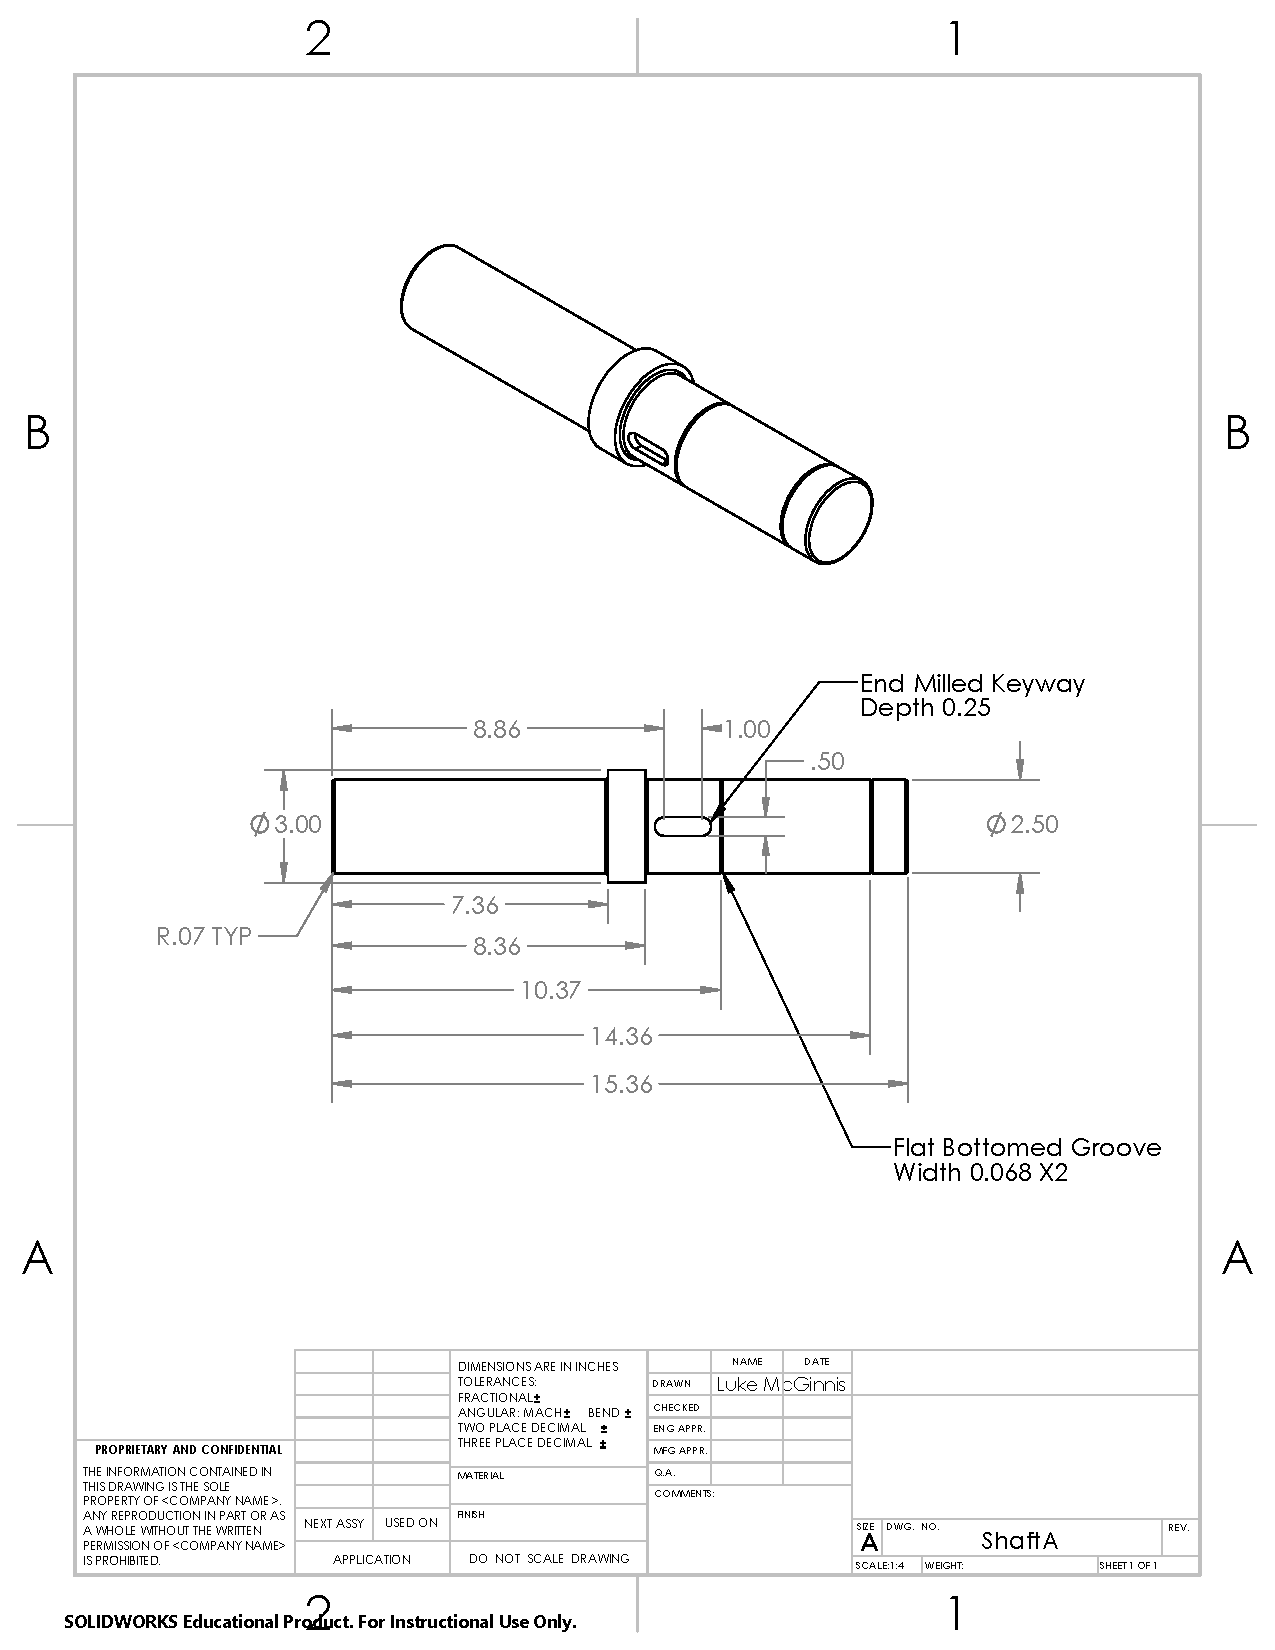
\includepdf[fitpaper=true, pages=-]{../cad/drawings/ShaftA.pdf}
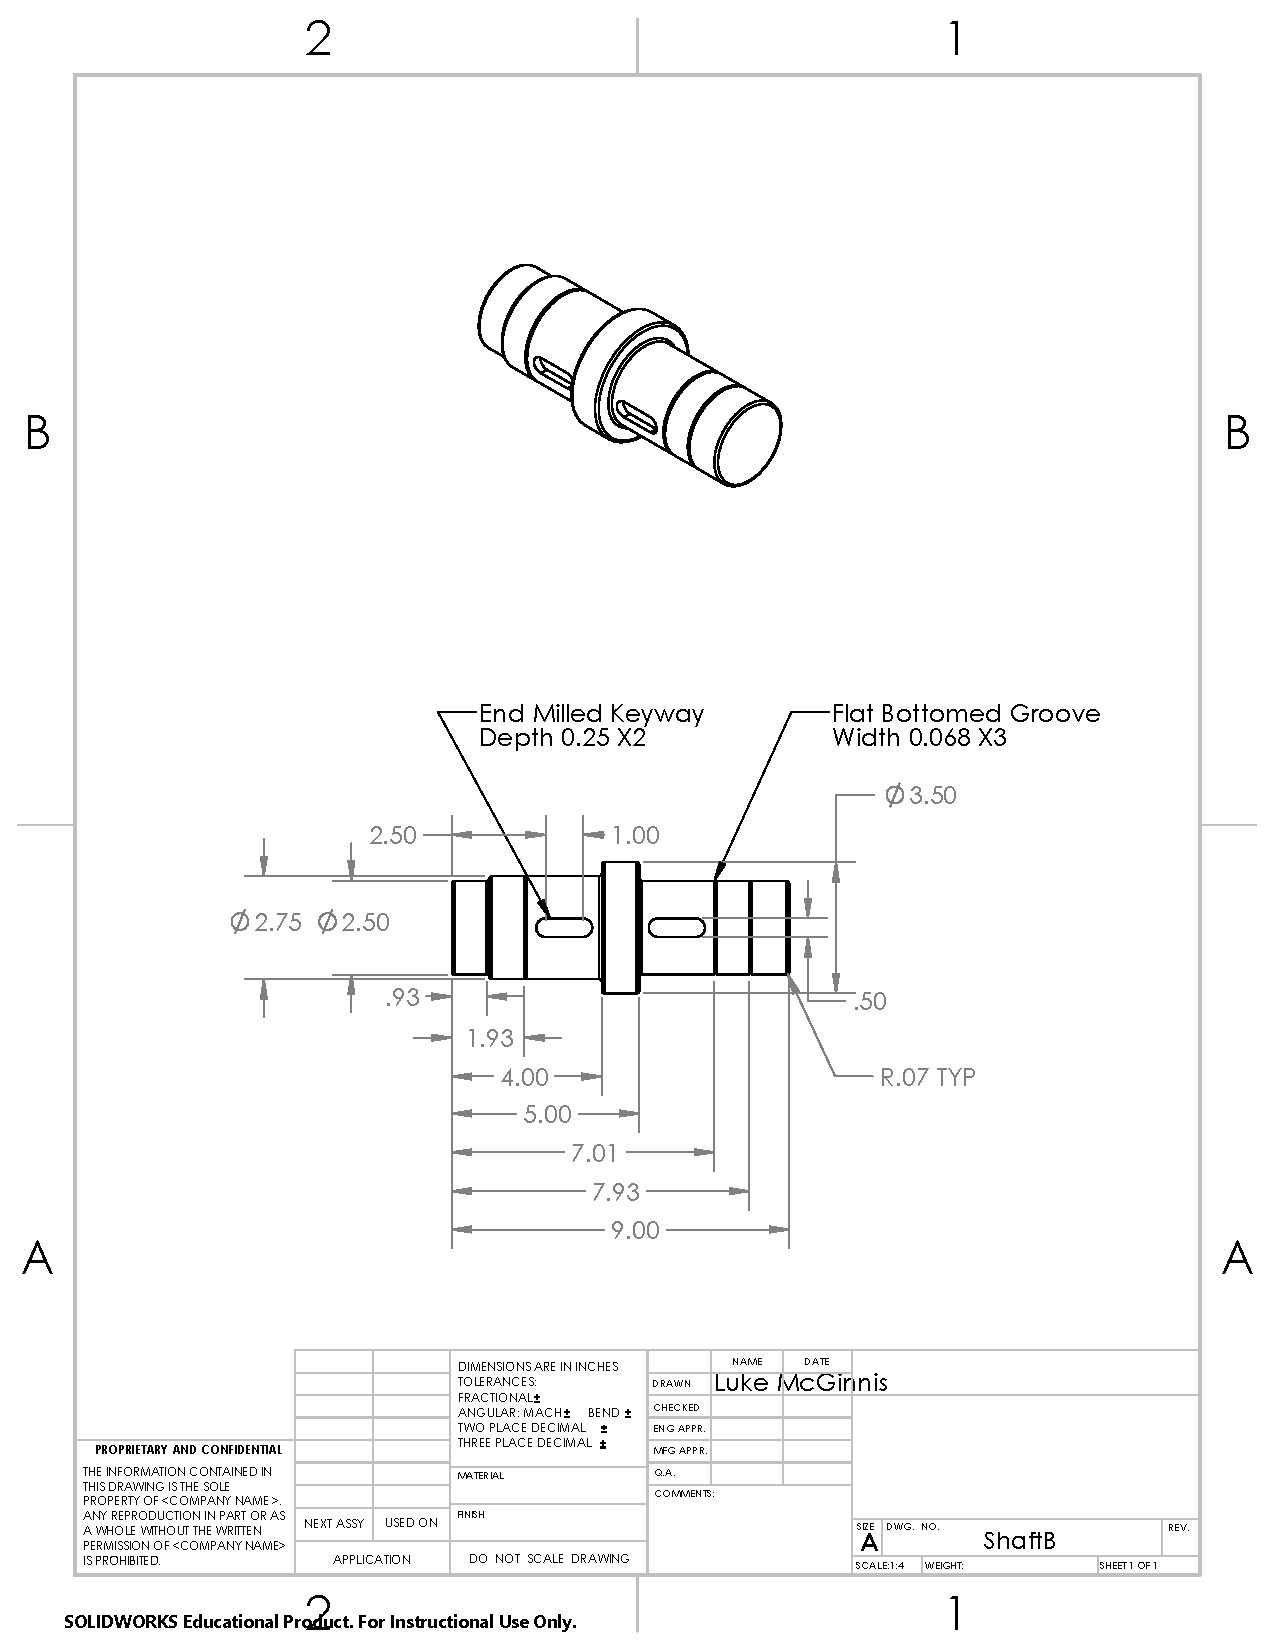
\includepdf[fitpaper=true, pages=-]{../cad/drawings/ShaftB.pdf}
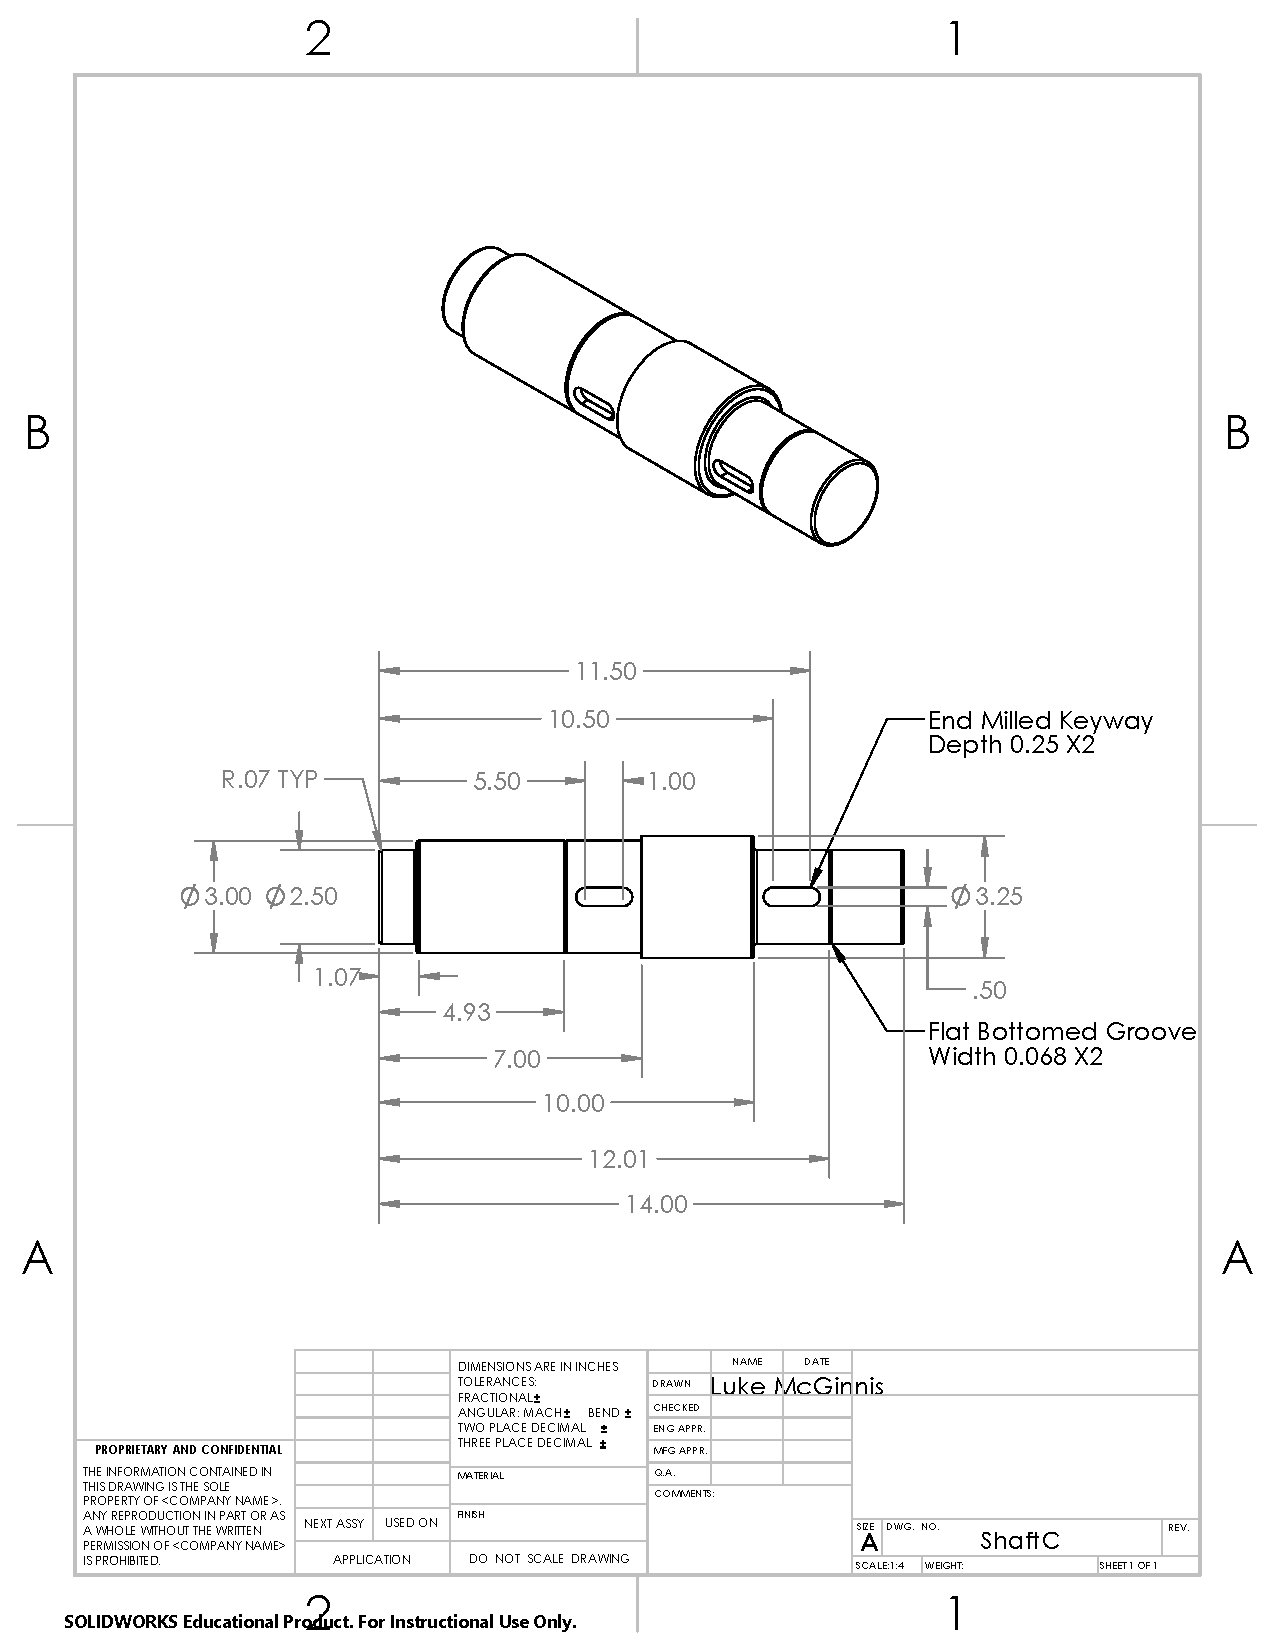
\includepdf[fitpaper=true, pages=-]{../cad/drawings/ShaftC.pdf}
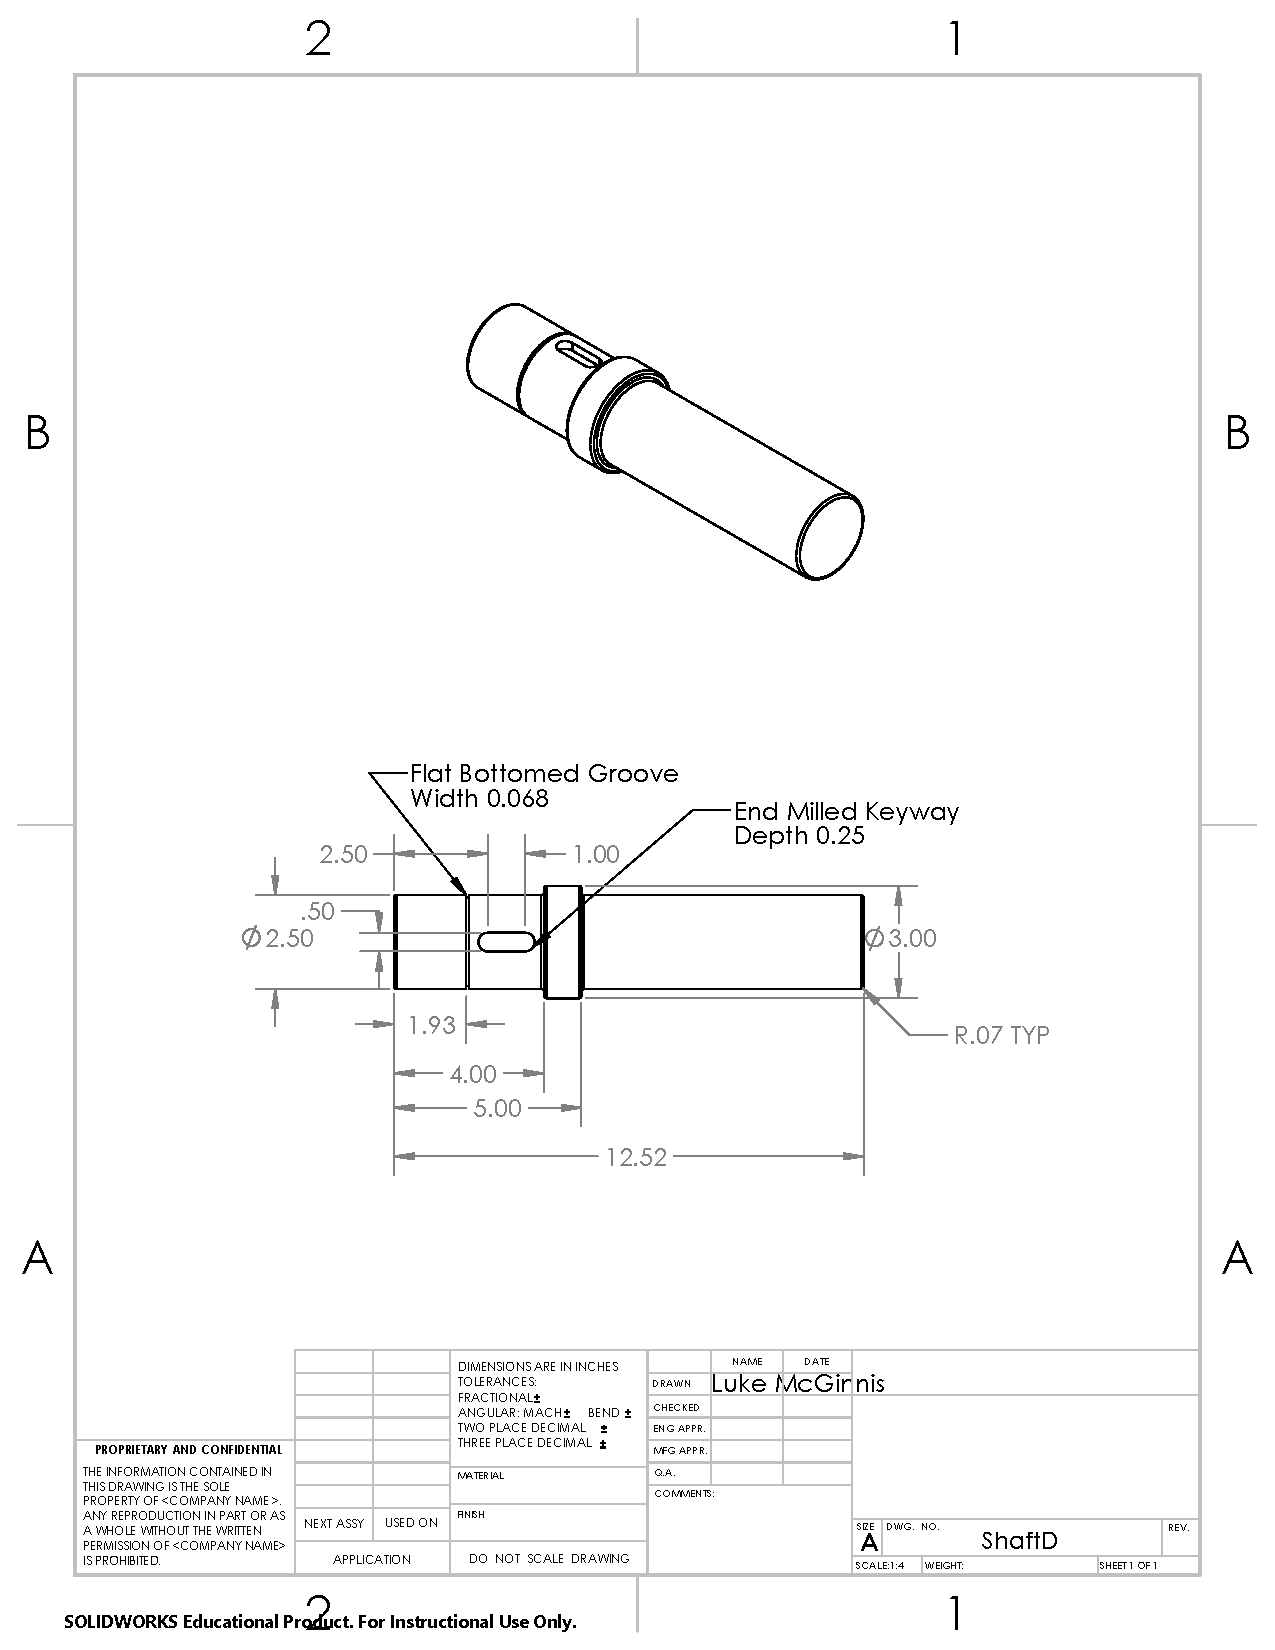
\includepdf[fitpaper=true, pages=-]{../cad/drawings/ShaftD.pdf}


\end{appendices}

\printbibliography

\end{document}

